%\chapter{Introdução}

A aprendizagem na área da computação envolve conhecimentos em conceitos abstratos, além de linguagens, exige alto nível de generalização, abstração e pensamento crítico. Desse modo, de acordo com \cite{InteractingFactorsThatPredict}, é imprescindível que haja tanto a dedicação por parte do aluno, quanto melhorias nos recursos voltados ao ensino, são necessárias alternativas que tornem os estudos mais eficientes e contribuam com a diminuição do número de reprovações em disciplinas introdutórias do curso. 

A tese de doutorado propõe a elaboração de uma Metodologia de correção e geração automática de feedbacks para submissões de respostas de alunos a exercícios computacionais do ciclo básico de computação. Esta metodologia prevê desde a definição de metadados necessários à criação de um exercícios, a definição das características que podem ser analisadas e o método para que os juízes online possam ao analisar a submissão responder com uma régua de sensibilidade a nota e um feedback adaptativo ao contexto do aluno. O objetivo é fornecer ao estudante um suporte claro ao seu autodesenvolvimento, indicando novas etapas do desenvolvimento para alcançar a resposta esperada.
Ao submeter uma resolução, a máquina de julgamento automático aplica testes à resolução, produzindo uma série de dados estatísticos sobre a resposta. Em seguida, uma máquina tomadora de decisão escolhe, baseada nesses resultados, qual seria a nota do aluno e a sugestão para que ele alcance a nota máxima. Essa abordagem envolve a criação de um sistema computacional que, além de avaliar a precisão das respostas com base em critérios rigorosos, é capaz de utilizar esses metadados para estabelecer uma regra de sensibilidade em relação à correção das atividades e oferecer sugestões de melhoria de forma heurística.


\begin{figure}
    \centering
    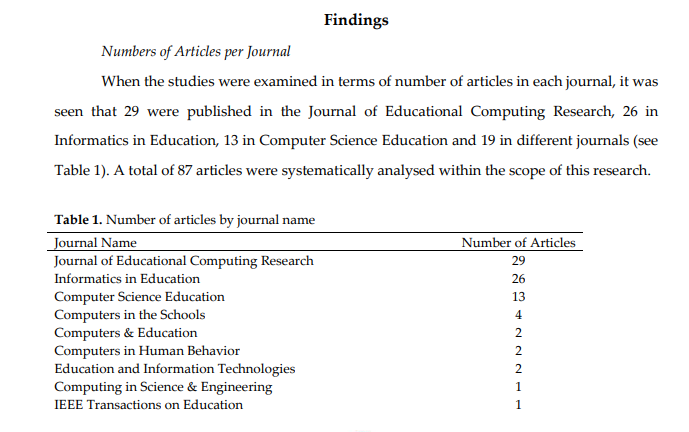
\includegraphics[width=1\linewidth]{qualificacao//figure/reaseach.png}
    \caption{Enter Caption}
    \label{fig:enter-label}

    \centering
    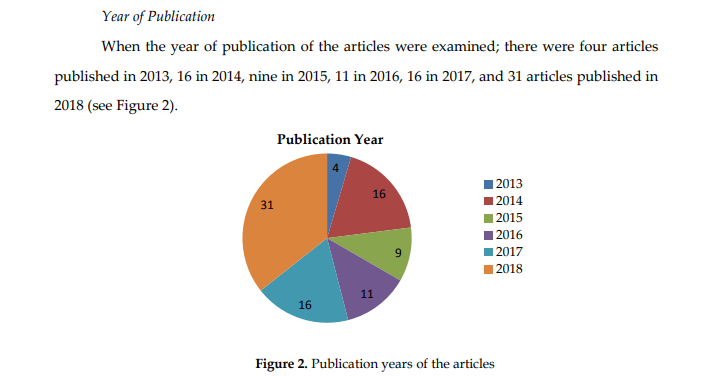
\includegraphics[width=1\linewidth]{qualificacao//figure/cap1-reasech2.png}
    \caption{Enter Caption}
    \label{fig:enter-label}
\end{figure}

\tresumo{Aprender Computação é difícil.}

\tresumo{Apresentar estudos que comprovam a investigação e desafios.}


\tresumo{Livro Computer Science Education Research}

 Dez áreas identificadas pelas autoras em relação à educação em ciências da computação:

\tresumo{Termo: Research Implications for Computer Science Education}

\begin{enumerate}
    \item Pensamento computacional: Inclui o desenvolvimento de habilidades e estratégias de resolução de problemas, abstração, decomposição e reconhecimento de padrões.
    \item Programação: Enfoca o ensino e a aprendizagem de conceitos e técnicas de programação, incluindo linguagens de programação, algoritmos e estruturas de dados.
    \item Laboratório: Refere-se à experiência prática em laboratório, onde os alunos podem explorar e aplicar os conceitos aprendidos em um ambiente prático.
    \item Computação e sociedade: Aborda questões éticas, legais e sociais relacionadas à computação, como privacidade, segurança, propriedade intelectual e impactos da tecnologia na sociedade.
    \item Fundamentos da ciência da computação: Envolve a compreensão dos princípios teóricos e conceituais da ciência da computação, como lógica, teoria dos autômatos, estruturas formais e complexidade.
    \item Estratégias de ensino e aprendizagem: Refere-se a abordagens e métodos de ensino eficazes, estratégias de avaliação, planejamento curricular e adaptação do ensino às necessidades dos alunos.
    \item Interface humano-computador: Concentra-se no design e na interação de sistemas computacionais com os usuários, incluindo usabilidade, design centrado no usuário e interação homem-máquina.
    \item Avaliação: Envolve a medição e avaliação do progresso dos alunos, incluindo técnicas de avaliação formativa e somativa, feedback e acompanhamento do desempenho.
    \item Comunicação: Refere-se às habilidades de comunicação oral e escrita na área da ciência da computação, incluindo relatórios técnicos, documentação de software e apresentações.
    \item Recursos e ferramentas de apoio: Inclui o acesso a recursos de aprendizagem, como livros, tutoriais, ambientes de programação, simuladores e ferramentas de suporte ao ensino.
\end{enumerate}


\tresumo{Citar que aprender precisa de um Guia e a Pedagogia já diz q é relevante.}

\tresumo{Ter um Tutor automatizado poderia ser incrível para auxiliar a aprendizagem. [aprender o quê? é importante delimitar o escopo]}

\tresumo{Será possível Criar um automatizado com critérios baseado nas ferramentas atuais? [a resposta em geral é ``sim'', mas você quer refinar essa pergunta, para que a sua proposta seja de fato a resposta para ela (e que a resposta não esteja já na literatura)]}


% Têm-se verificado nas disciplinas de Linguagens e Lógica de programação uma alta taxa de reprovação ou evasão, \cite{d_2008} apresenta dados sobre o Instituto de Ensino Superior (IES) em que a taxa de desistência ou reprovação chega a 60\% nas disciplinas introdutórias de programação.

% Não vamos discutir aqui as várias metodologias para analisar e justificar as taxas de reprovação, entretanto, fundamentado nos trabalhos de \cite{g_m_2013}, \cite{g_h_m_2008}, \cite{l_a_j_2005}, \cite{d_2008}, \cite{l_2000} \cite{b_c_2005}, \cite{b_2008} destacaremos algumas possíveis causas como: a dificuldades na compreensão e aplicação de conceitos básicos de computação; dificuldade em lidar com a abstração e conceitos de lógica; foco no aprendizado técnico da linguagem (sintaxe e ambiente) em detrimento da lógica computacional; utilização de metodologias que criam uma ruptura na forma com a qual o aluno aprende até então. 

% \cite{g_h_m_2008} aborda dificuldades nos processo de ensino de programação e destaca que a escolha de linguagem de programação ou uso de ferramentas audiovisuais não ajuda a resolver o problema como um todo, pois cada aluno possui um perfil de aprendizado diferente, sendo favorecido ou desfavorecido por tais escolhas. Ele conclui e \cite{d_2008} também reforça,  que uma metodologia/ferramenta que motive o aluno e o acompanhe durante todo o processo de aprendizado é a melhor proposta. a necessidade de motivar o aluno, além da utilização das ferramentas e metodologias. 

% \cite{l_a_j_2005} aplicaram questionários a alunos e professores, investigando dificuldades no processo de ensino/aprendizagem de programação, e concluíram que questões técnicas como escolha de linguagem de programação não mudam as dificuldades sentidas pelos alunos. Perceberam que quanto mais abstrato um tema de programação é, maior é a dificuldade sentida pelos alunos em aprender o mesmo. 
% \cite{r_f_m_n_g_2010} afirmam que independentemente da metodologia utilizada, lógica de programação é requisito fundamental nos cursos de computação, sendo base no desenvolvimento de raciocínio lógico e construção de algoritmos corretos.

% \cite{h_k_s_2014} constataram que o ensino é alvo das aplicações de \textit{gamification}, e através de uma revisão literária, conseguiram concluir que o seu uso motivou positivamente os alunos. \cite{m_k_h_2018} confirmaram tal conclusão, apresentando uma revisão literária de trabalhos que usaram a \textit{gamification} no ensino, mas que apresentaram dados empíricos. Foi identificado que poucos trabalhos têm mensurado o impacto da \textit{gamification} no processo de aprendizagem; estes estão mais voltados para avaliação de motivação e engajamento.

% Existem diversas competições de programação como: \textit{International Olympiad in Informatics} (IOI) voltadas tanto para alunos do ensino médio; o \textit{International Collegiate Programming Contest} (ICPC), promovido pela \textit{Association for Computing Machinery} (ACM); e a Maratona de Programação promovida pela Sociedade Brasileira de Computação no Brasil como parte da ICPC. Estes ambientes competitivos tem aumentado de forma constante o número de participantes a cada ano, demonstrando o interesse dos estudantes, como pode ser exemplificado na Figura \ref{fig:acm-student-participation} retirado do relatório anual \cite{icpc_2020}.

% \begin{figure}[h]
% 	\caption{\label{fig:acm-student-participation}Crescimento da participação de estudantes em competições da ICPC.}
% 	\centering
% 		\includegraphics[width=1.0\textwidth]{Base TCC/imagens/cap1-acm-student-participation.png}
% 	\legend{Fonte: (ICPC, 2020).}
% \end{figure}

% Além destas, destacam-se também, competições livres que ocorrem pela internet, realizadas por empresas ou por sites que disponibilizam problemas online com corretores automáticos, úteis como treino para outras competições, apesar de normalmente não oferecerem premiações. 

% Partimos então de uma percepção de que como o interesse pelas competições de programação aumentando, vêm sendo desenvolvidas diversas ferramentas e repositórios de problemas que buscam auxiliar e contribuir com o aprendizado de estudantes tanto para treinamento quanto aprendizado da computação.



% Apesar de citar o termo tutor inteligente, ele não é o objeto de estudo deste trabalho onde estamos buscando ainda um formalismo para que novas possibilidades possam ser desenvolvidas em no ambiente educacional de ensino. 

% Propomos estudar uma forma para formalizar a definição de problemas computacionais que serão julgados por técnicas de sistemas Julgadores Automáticos. Entretanto tal formalização busca fornecer dados suficientes para o fornecimento de feedback automático relevante ao processo educacional de aprendizado de Lógicas e Técnicas computacionais. 

% Este feedback é usado como um artefato que enriquece as possibilidades do processo de gamificação já pré existente nas ferramentas atuais de competição.
 

 %   Exemplo de nota de rodapé \footnote{Aqui está uma nota de rodapé e uma url: \url{https://dcc.ufmg.br}}.

    
\section{Motivação}

    \tresumo{Criar uma IA que seja consultiva ao adiquirir[adquirir] um conhecimento em linguagem natural parece ser um sonho}
    
\section{Definições Preliminares}


\begin{itemize}
    \item Vendo o crescimento supostamente voluntário e orgânico, da participação dos estudantes em eventos competitivos de computação com feedback instantâneo, acreditamos que são estudantes sofrem alguma forma de estímulo pela metodologia;
    
    % \item A partir dos estudos estes os estímulos que provocam a desistencia dos estudos em computação é a dificuldade em encontrar saídas em problemas o auxilio por computador pode ser uma alternetiva.
 
     \item Estudantes e professores da área de computação podem se beneficiar ao utilizar tais sistemas de forma adequada;
 
    \item Os repositórios de problemas mais famosos, não tem características de ensino, pois suas bases de conhecimento foram focadas exclusivamente em processo de treinamento, sendo deficientes de características educacionais;
 
    \item Um dos pontos deficitários dos problemas disponíveis são suas capacidades de feedback e classificação educacional, sendo que precisam que precisam de mais metadados para atender possibilidades mais amplas;

    \item Com uma definição de quais metadados proporcionariam melhores recursos educacionais, principalmente focando no feedback, os ambientes poderiam utilizar-se de seus elementos gameficados subutilizados e fornecer ao aluno uma experiência nova que se aproximaria do conceito computacional de um tutor inteligente.
\end{itemize}

    \tresumo{As linguagens de programação são formais, e possuiem[possuem] um ambiente fechado de execução }
    
    \tresumo{Já existem ferramentas capazes de julgar soluções do ponto de vista de entrada correta e saída correta, além de avaliar vários critérios de simulações de resposta }
    
\section{Problemática}
    
    \tresumo{Citar que aprender precisa de um Guia e a Pedagogia já diz q é relevante.}
    
\section{Objetivos}\label{sec:objetivos}

Com base na contextualização acima, este trabalho visa atacar um dos principais problemas relacionados, que é a falta de feedback do aluno sobre o conhecimento adquirido no momento de submissão de um exercício. Mais especificamente, deverão ser definidas diretivas, algorítimos e metadados necessários para que ferramentas automáticas possam além de responder sobre a assertividade do aluno na resposta, possa sugerir e guiar o aluno de forma autônoma. Com isso, define-se o seguinte objetivo geral:

\medskip
\noindent \fbox{%
  \parbox{1.0\textwidth}{%
  \textbf{Objetivo Geral:} [determinar se] Usando ferramentas classificadas como Juízes Onlines propor diretrizes para que elas possam fornecer ao usuário uma análise da resposta de um programa computacional submetido a um problema e sugerir de forma assertiva e inteligente sugestões sobre a estratégia lógica de um aluno ao fazer um exercício. Buscando seu aprimoramento autônomo. Heuristica deterministca.
  \par
  }%
}
\medskip

x`  Entretanto para se chegar a este objetivo será necessário fazer alguns passos representados pelos objetivos específicos.


Desenvolver um sistema

Fazer um protípo

Ensaios de experimento

estudo de caso

*Formalizar metadados (Características comuns, e elementos de suporte) para o recorte especific. par dar o retorno

Estudar viabilidade, revisão, de feedback a ser dados.  baseado nisso propor o modelo para este tipo de erro.

\medskip
\noindent \fbox{%
  \parbox{1.0\textwidth}{%
  \textbf{Objetivo Específico 1} (baseado em dados de análises prévias) Realizar uma análise das categorias de erros mais comuns aos estudantes especificamente à programação estruturada e com aplicação de ordem de complexidade.
  \par
  }%
}
\medskip

Vou contruir uma ferramente que será construída para avaliar.

\medskip
\noindent \fbox{%
  \parbox{1.0\textwidth}{%
  \textbf{Objetivo Específico 2} Realizar uma análise das possíveis características a serem documentada como meta dados tanto do exercício quanto dos casos de testes relacionados.
  \par
  }%
}
\medskip

\tresumo{LEvantar teses em portugues sobre estes tipo de trabalho}

  % \textbf{Objetivo Geral} Usando ferramentas classificadas como Juiz Automáticos criar diretrizes para que elas possam fornecer ao usuário respostas fazerem diagnósticos de "certo" ou "errado" sobre uma solução fornecem informações lógicas e exatas sobre a execução. Unificando estas análises lógicas e exatas com meta dados sobre o problema e seus casos de testes queremos provar ser possível inferir com certo grau de certeza sugestões sobre a estratégia lógica de um aluno ao fazer um exercício. Buscando seu aprimoramento

Apresentar um framework formal capaz de dar à máquina a capacidade de dar um feedback acertivo e compatível com o processo de aprendizado e treinamento educacional.
 \textit{gamification} no processo de aprendizado de programação.

Objetivos específicos:
\begin{itemize}
\item Definir um modelo formal para a definições de metadados de problemas para computação competitiva educacional com foco na geração de feedback com fim educacional e de aprendizagem

\item Apresentar uma proposta algorítmica que avalia o modelo e demonstra as formas de geração de feedback esperados.

\item Projetar uma arquitetura de plataforma que utilize tais técnicas e implementar um protótipo;

\item Levantar na literatura as possibilidades de feedback em sistemas de julgamento automático  adequados ao aprendizado com programação, e selecionar um conjunto destas características;

\item Justificar estes itens de feedback alinhando com os elementos de gameficação presentes na literatura;

\item Avaliar através de experimentos o impacto da técnica de \textit{gamification} no processo de aprendizagem de programação junto com a modelagem de exercícios.
\end{itemize}

        
\section{Contribuições}

    Visando atingir os objetivos específicos apresentados na Seção \ref{sec:objetivos}, esta seção define e destaca as duas principais contribuições deste trabalho. A primeira contribuição envolve o objetivo específico 1 enunciado na Seção \ref{sec:objetivos}, focando em conteúdo não segmentado e cuja qualidade não varia ao longo do tempo:
        
    \medskip\noindent \fbox{%
      \parbox{1.0\textwidth}{%
      \textbf{Contribuição 1:} ....
      \par
      }%
    }\medskip

    \medskip\noindent \fbox{%
      \parbox{1.0\textwidth}{%
      \textbf{Contribuição 2:} ....
      \par
      }%
    }\medskip
\section{Organização do Trabalho}
        dsd
               
Exemplo de nota de rodapé \footnote{Aqui está uma nota de rodapé e uma url: \url{https://dcc.ufmg.br}}.
	